%%%%%%
%
% $Autor: Wings $
% $Datum: 2020-01-18 11:15:45Z $
% $Pfad: githubtemplate/Template/Presentations/Template/slides/rename.tex $
% $Version: 4620 $
%
%
% !TeX encoding = utf8
% !TeX root = Rename
%
%%%%%%

\Mysection{Leopard Imaging IMX219 MIPI FF NANO 8.08 MP Camera}
\STANDARD{Leopard Imaging IMX219 MIPI FF NANO 8.08 MP Camera}
{
	
% TODO: \usepackage{graphicx} required
\begin{figure}
	\centering
	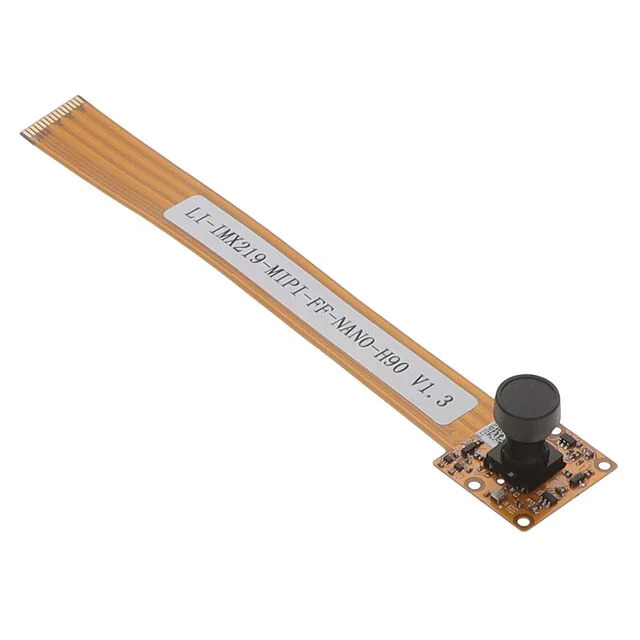
\includegraphics[width=0.4\linewidth]{images/LIIMX219}
	\caption{Leopard Imaging IMX219 MIPI FF NANO 8.08 MP Camera}
	\label{fig:liimx219}
\end{figure}


}
\STANDARD{Leopard Imaging IMX219 MIPI FF NANO 8.08 MP Camera}{
	\centering
	\begin{itemize}
		\item \textbf{Sensor}: Sony IMX219 CMOS color sensor (8.08 MP)
		\item \textbf{Resolution}: $3280 \times 2464$ active pixels
		\item \textbf{Pixel Size}: $1.12\,\mu m \times 1.12\,\mu m$
		\item \textbf{Optics}: Fixed-focus lens (H90 / H136 / H145 variants)
		\item \textbf{Field of View}: $90^\circ$, $136^\circ$, or $145^\circ$ (horizontal)
		\item \textbf{Interface}: 2-lane MIPI CSI-2
		\item \textbf{Frame Rate}: Up to 21 fps at full resolution
		\item \textbf{Platform}: NVIDIA Jetson Nano
	\end{itemize}
}

\STANDARD{Hardware Connection: IMX219 to Jetson Nano}{
	\centering
	\begin{enumerate}
		\item Power off the Jetson Nano.
		\item Connect the IMX219 camera ribbon cable to the CSI connector (CAM0).
		\item Ensure correct orientation of the FPC cable (contacts facing inward).
		\item Power on the Jetson Nano and verify camera detection.
	\end{enumerate}
}

\STANDARD{Camera Indicators and Status Signals}{
	\centering
	\begin{itemize}
		\item \textbf{Power Indicator}: The IMX219 camera module does not include a dedicated onboard LED; power status is inferred from successful CSI initialization.
		\item \textbf{Activity Indication}: Camera activity is indicated at the system level by successful frame acquisition through V4L2, OpenCV, or GStreamer pipelines.
		\item \textbf{Driver-Level Feedback}: Kernel logs (\texttt{dmesg}) and device enumeration (\texttt{/dev/video0}) confirm sensor detection and readiness.
		\item \textbf{Error Indication}: Absence of video devices or capture failures indicate improper ribbon orientation, power issues, or driver misconfiguration.
	\end{itemize}
}


\STANDARD{Camera Calibration Procedure}{
	\centering
	\begin{enumerate}
		\item Print a checkerboard calibration target.
		\item Capture multiple images at different orientations.
		\item Detect checkerboard corners using OpenCV.
		\item Estimate intrinsic parameters and distortion coefficients.
		\item Store calibration parameters for runtime correction.
	\end{enumerate}
}
	
\STANDARD{IMX219 Camera Module Imports}{
		\lstinputlisting[
		language=Python,
		style=mystyle,
		firstline=1,
		firstnumber=1,
		caption={Module description and imports (IMX219Cam.py)}
		]{Code/IMX219Cam.py}
}

\Mysection{Next Steps}
\STANDARD{Next Steps}{
	\begin{itemize}
		\item Integrate the IMX219 camera pipeline into a ROS~2 node using \texttt{rclpy}
		\item Publish image frames as \texttt{sensor\_msgs/Image} topics
		\item Add \texttt{camera\_info} publishing using calibration parameters
		\item Enable hardware-accelerated pipelines using GStreamer on Jetson
		\item Perform extrinsic calibration for multi-sensor setups
		\item Connect the camera feed to Nav2 perception or SLAM pipelines
		\item Containerize the camera stack using Docker for reproducibility
	\end{itemize}
}



